\documentclass[11pt]{article}

% === Page geometry ===
\usepackage[margin=1in]{geometry}

% === Colors (must be before tikz/pgfplots) ===
\usepackage[dvipsnames]{xcolor}

% === Math and symbols ===
\usepackage{amsmath, amssymb}

% === Tables ===
\usepackage{array, booktabs, multirow}

% === Algorithms ===
\usepackage[ruled,vlined,linesnumbered]{algorithm2e}

% === Graphics ===
\usepackage{tikz}
\usetikzlibrary{positioning, shapes.geometric, arrows.meta, fit, calc, backgrounds, decorations.pathreplacing}
\usepackage{pgfplots}
\pgfplotsset{compat=1.18}

% === Citations ===
\usepackage[numbers,sort&compress]{natbib}

% === Hyperlinks ===
\usepackage[colorlinks=true,linkcolor=blue!60!black,citecolor=blue!60!black,urlcolor=teal]{hyperref}

% === Figures ===
\usepackage{subcaption}
\usepackage{graphicx}

% === Misc ===
\usepackage{enumitem}
\usepackage{microtype}

% === Title formatting ===
\usepackage{titlesec}
\titleformat{\section}{\large\bfseries}{\thesection}{1em}{}
\titleformat{\subsection}{\normalsize\bfseries}{\thesubsection}{1em}{}

% === Line spacing ===
\usepackage{setspace}
\setstretch{1.15}

% === Header ===
\usepackage{fancyhdr}
\pagestyle{fancy}
\fancyhf{}
\rhead{\small\thepage}
\lhead{\small Nous: Cognitive Priors for LLM Agents}
\renewcommand{\headrulewidth}{0.4pt}

% === Custom commands ===
\newcommand{\nous}{\textsc{Nous}}
\newcommand{\eg}{e.g.}
\newcommand{\ie}{i.e.}
\newcommand{\cf}{cf.}

\title{\textbf{Nous: Extracting and Injecting Cognitive Priors\\for Diverse LLM Agents}}

\author{
  Haowei Qian \\
  Independent Researcher \\
  \texttt{haowei0509@gmail.com}
}

\date{}

\begin{document}

\maketitle

% ============================================================
% ABSTRACT
% ============================================================
\begin{abstract}
As large language model (LLM) agents proliferate in prediction markets, financial analysis, and collective decision-making, they introduce a systemic risk: \emph{cognitive monoculture}. Agents built on the same foundation models, trained on overlapping data, and aligned through similar procedures converge on homogeneous reasoning patterns, undermining the epistemic diversity that makes collective intelligence possible. We argue that this convergence is a structural consequence of training objectives that learn mean-field approximations of human cognition, systematically averaging out individual cognitive variation. We identify the missing architectural layer as \emph{cognitive preprocessing}---the pre-reasoning information processing that shapes which signals an agent attends to, how it perceives risk, and how quickly it updates beliefs. We present \nous{}, a framework consisting of: (1)~an eight-dimensional cognitive schema organized in a Core-Shell-Membrane architecture with graded stability; (2)~a behavioral extraction pipeline that infers structured cognitive profiles from prediction market activity using Prospect Theory curve fitting, attention decay models, and belief update analysis; (3)~a structure-to-narrative translator that converts parametric profiles into natural-language system prompts; and (4)~an injection mechanism that installs these cognitive priors as the foundational layer of an agent's prompt. In controlled experiments using three synthetic personas, five test scenarios, and three models (Qwen3-32B, DeepSeek-R1-32B, Llama~3.1-8B), preliminary results indicate that \nous{}-injected agents produce judgment-level differentiation---not merely stylistic variation---on 4 out of 5 tasks across all models, with textual trigram Jaccard distances of 0.575--0.666. A second-generation continuous translator achieves a 16.3\% mean diversity improvement over the original threshold-based translator, matching handwritten persona baselines on textual diversity while remaining fully automated, though handwritten personas retain an advantage on structured-output metrics. Cross-language comparison using the v1 translator reveals that English injection achieves deeper cognitive penetration than Chinese on Qwen3-32B. We discuss the ``correct answer bias'' phenomenon whereby LLM safety alignment overrides injected priors on tasks with socially consensual answers, and argue that this self-constraining property is a feature rather than a limitation. All code and experimental data are publicly available.
\end{abstract}

\vspace{0.5em}
\noindent\textbf{Keywords:} cognitive diversity, prediction markets, LLM agents, cognitive priors, epistemic monoculture, behavioral extraction

% ============================================================
% 1. INTRODUCTION
% ============================================================
\section{Introduction}
\label{sec:intro}

The deployment of autonomous LLM agents in information-rich domains---prediction markets~\citep{hanson2003combinatorial}, investment analysis, and collective decision-making---is accelerating rapidly. Agent frameworks such as Generative Agents~\citep{park2023generative} and multi-agent debate systems~\citep{du2023debate} demonstrate increasingly sophisticated reasoning capabilities. However, this expansion carries a structural risk that has received insufficient attention: the erosion of \emph{epistemic diversity} in agent populations.

\citet{surowiecki2004wisdom} identified four conditions necessary for collective intelligence: \emph{diversity of opinion}, \emph{independence of judgment}, \emph{decentralization}, and \emph{aggregation mechanisms}. Prediction markets satisfy the fourth condition through price discovery, and traditionally approximate the first three through human cognitive heterogeneity. However, when agents replace or supplement human participants, all three enabling conditions are systematically undermined:

\begin{itemize}[leftmargin=*,itemsep=2pt]
    \item \textbf{Diversity collapses.} The market is dominated by a small number of foundation models (GPT, Claude, Gemini, Llama, DeepSeek), trained on heavily overlapping corpora. One thousand agents may represent only 3--5 genuinely independent reasoning pathways.
    \item \textbf{Independence is illusory.} Agents consuming the same news APIs, using similar prompt engineering patterns, and observing the same price signals create correlated information processing, not independent judgment.
    \item \textbf{Decentralization is superficial.} Physical distribution across servers masks cognitive centralization in a handful of model providers.
\end{itemize}

This \emph{cognitive monoculture}---a term we adapt from the algorithmic monoculture identified by \citet{kleinberg2021algorithmic}---produces three dangerous consequences: artificially high confidence in systematically biased estimates, correlated tail risks where all agents fail simultaneously on out-of-distribution events, and vulnerability to adversarial attacks that exploit shared model weaknesses.

We argue that the missing architectural component is not stronger reasoning or better tools, but a layer of \emph{cognitive preprocessing}---the pre-reasoning information processing that determines what an agent attends to, how it perceives risk, and how readily it updates beliefs. In human cognition, this layer corresponds to what \citet{klein1998sources} calls recognition-primed decision-making, what \citet{kahneman2011thinking} characterizes as System~1 processing, and what \citet{damasio1994descartes} theorizes as somatic markers. It is the computational substrate of intuition: structured, individual, and consequential for judgment.

This paper presents \nous{}, a framework for extracting, representing, and injecting human cognitive priors into LLM agents. Our contributions are:

\begin{enumerate}[leftmargin=*,itemsep=2pt]
    \item \textbf{The \nous{} Schema}: an eight-dimensional cognitive profile organized in a three-layer Core-Shell-Membrane architecture, grounded in behavioral economics, expert intuition research, and Bayesian cognition.
    \item \textbf{A behavioral extraction pipeline}: algorithms that infer cognitive parameters from prediction market behavior, including Prospect Theory curve fitting for risk perception and exponential decay models for attention allocation.
    \item \textbf{A structure-to-narrative injection mechanism}: a translator that converts parametric profiles into natural-language cognitive instructions, and an injector that installs them as the foundational prompt layer.
    \item \textbf{Preliminary experimental evidence}: proof-of-concept results demonstrating that injection produces judgment-level differentiation across synthetic personas, with cross-language analysis revealing interaction effects between injection language and cognitive penetration depth.
\end{enumerate}

We emphasize that the current work constitutes an \emph{architectural proposal with preliminary validation}. The extraction pipeline has been tested only on synthetic behavioral data, and the injection experiments use a limited set of personas and questions. Validation on real prediction market data is the highest-priority next step (Section~\ref{sec:discussion}).

The remainder of this paper is organized as follows. Section~\ref{sec:related} surveys related work across human decision-making, agent personalization, and prediction market theory. Section~\ref{sec:priors} formally defines cognitive priors and the \nous{} Schema. Section~\ref{sec:extraction} presents the extraction pipeline. Section~\ref{sec:injection} describes the translation and injection mechanism. Section~\ref{sec:experiments} reports experimental results. Section~\ref{sec:discussion} discusses implications and limitations. Section~\ref{sec:conclusion} concludes.


% ============================================================
% 2. RELATED WORK
% ============================================================
\section{Related Work}
\label{sec:related}

\subsection{Human Decision-Making and Intuition}

The theoretical foundations of \nous{} draw from three decades of research on human judgment under uncertainty. \citet{kahneman1979prospect} established that human risk perception follows an asymmetric value function with individual-specific curvature parameters ($\alpha$, $\beta$) and loss aversion coefficient ($\lambda$), providing the mathematical basis for our risk perception dimension. \citet{kahneman2011thinking} formalized the distinction between fast, intuitive (System~1) and slow, deliberative (System~2) processing, which maps directly to our cognitive style dimension.

\citet{klein1998sources} demonstrated through naturalistic decision-making studies that expert intuition operates through recognition-primed decision (RPD)---rapid pattern matching against accumulated experience. The critical insight for our work is that expert intuition is \emph{structured and describable}, not mystical. \citet{kahneman2009conditions} reconciled the heuristics-and-biases tradition with the naturalistic decision-making school, establishing that valid intuitive expertise requires both a high-validity environment and sufficient practice---conditions that prediction markets are designed to approximate.

\citet{tetlock2015superforecasting} identified the cognitive traits of ``superforecasters'': actively open-minded thinking, frequent belief updating, granular probabilistic reasoning, and the fox-like integration of diverse information sources (in contrast to hedgehog-like reliance on a single explanatory framework~\citep{tetlock2005expert}). These traits directly inform the belief update inertia and cognitive style dimensions of our schema.

\subsection{AI Agent Personalization}

Recent work has explored personalization of LLM agents through various mechanisms. \citet{park2023generative} introduced generative agents with memory, reflection, and planning modules, but personality is specified through hand-written character descriptions rather than extracted from behavioral data. \citet{shanahan2023role} analyzed role-playing with LLMs, showing that persona prompting produces surface-level behavioral changes. \citet{salewski2024context} demonstrated that in-context impersonation reveals model biases rather than genuine cognitive diversity.

Commercial systems (Character.ai, Personal.ai) focus on personality simulation or knowledge retrieval, not on cognitive preprocessing. The gap we address is the absence of a principled pipeline from \emph{behavioral observation} to \emph{structured cognitive profile} to \emph{verifiable injection}.

\paragraph{Recent cognitive prior approaches.}
A growing body of work explores cognitive dimensions of LLM agents, though from different angles than \nous{}. At the single-agent level, \citet{bao2025conflictaware} address logical reasoning under contradictory evidence through a dual-process architecture, and \citet{yang2026thinkfastslow} introduce CogRouter, which dynamically adapts cognitive depth at each reasoning step within a single agent across four hierarchical levels grounded in ACT-R theory. \citet{zhu2024bootstrapping} bootstrap cognitive architectures for embodied agents using LLM knowledge, demonstrating that cognitive structure can be externalized from the model itself. At the evaluation level, \citet{chen2025causal} show that language agents mirror human causal reasoning biases---exhibiting systematic biases in causal structure learning that highlight the cognitive heterogeneity present in human reasoning. \citet{wang2025beyondbias} propose a multi-cognition agentic framework that assigns diverse cognitive perspectives to mitigate forecasting biases. \citet{zhu2024eliciting} demonstrate that LLMs encode recoverable probabilistic priors that qualitatively align with human priors, extractable via iterated in-context learning.

These works treat cognitive characteristics as either \emph{universal architectural features} (reasoning depth, logical consistency) or \emph{population-level biases to be measured or mitigated}. None extracts \emph{individual-specific} cognitive profiles from behavioral data, nor injects them as portable external modules to create inter-agent diversity. Our work is orthogonal: we do not seek to improve how agents reason, but to ensure that different agents reason \emph{differently}.

\subsection{Multi-Agent Diversity}

\citet{du2023debate} showed that multi-agent debate improves factuality, but their diversity comes from stochastic sampling, not from structured cognitive differences. Ensemble methods~\citep{lakshminarayanan2017simple} achieve diversity through architectural or training variation. \citet{hong2004groups} showed formally (under specific conditions) that diverse problem-solving groups can outperform groups of high-ability individuals---a result that motivates restoring cognitive diversity in agent populations.

\subsection{Prediction Markets and Information Aggregation}

Prediction markets aggregate distributed information through price discovery~\citep{wolfers2004prediction, arrow2008promise}. \citet{reichenbach2025polymarket} analyzed trading patterns on Polymarket, finding evidence of skill heterogeneity among participants. \citet{prelec2004bayesian} introduced the Bayesian Truth Serum for eliciting honest subjective judgments, and \citet{prelec2017solution} extended this to crowd wisdom problems. These works establish prediction markets as high-validity environments where cognitive differences produce measurable behavioral signatures.

\paragraph{Signal extraction methodology.}
\citet{madrigalcianci2026bayesian} formalize prediction markets as Bayesian inverse problems, inferring latent variables from price-volume histories. Their observation model introduces a latent mixture of trader types whose likelihood class encompasses informed and uninformed trading, heavy-tailed microstructure noise, and manipulative flow. This decomposition is directly relevant to \nous{} extraction: only informed flow constitutes valid cognitive signal, and noise filtering is critical for extraction quality.

\citet{shahabi2026truthtensor} evaluate LLMs as human-imitation systems anchored to live prediction markets, measuring how model forecasts diverge from human-calibrated baselines in calibration, drift, and risk-sensitivity. This is the inverse of our approach: where TruthTensor uses human market behavior as the ground truth to evaluate LLMs, \nous{} extracts cognitive priors from human behavior and injects them into LLMs to restore behavioral diversity. The distinction reflects a deeper architectural choice---TruthTensor measures how well LLMs approximate human forecasting behavior, while \nous{} seeks to make different LLM agents \emph{unlike each other}.

\paragraph{Incentive alignment.}
Honest reporting is a prerequisite for reliable cognitive extraction. \citet{prelec2004bayesian} designed the Bayesian Truth Serum (BTS) for scenarios lacking objective verification, incentivizing truthful subjective reports through a scoring rule that rewards ``surprisingly common'' answers. However, in prediction markets, BTS is largely redundant: participants wager real capital on their beliefs, providing the strongest possible incentive for honest expression---people do not bet against their genuine convictions with real money. This economic incentive alignment is a key reason we selected prediction markets as the extraction interface, rather than survey instruments or self-report questionnaires that require mechanisms like BTS to elicit honest responses.

\paragraph{Empirical evidence for extractable cognitive differences.}
Analysis of Polymarket trading data~\citep{reichenbach2025polymarket} reveals that approximately 30\% of traders achieve positive returns and that high-performing traders exhibit skill persistence across time periods. This finding provides empirical support for extractable ``cognitive dividends''---stable individual differences in information processing that produce systematically better predictions. However, the same data reveals a systematic YES bias: participants tend to overestimate the probability of positive outcomes. This bias, if unaccounted for, would contaminate the risk perception dimension of \nous{} extraction by inflating $\alpha$ estimates for users who are simply participating in a biased market. The current implementation does not correct for YES bias; we note this as a limitation (Section~\ref{sec:discussion}).

\paragraph{Gap statement.} No prior work addresses the full pipeline: extracting structured cognitive priors from prediction market behavior, organizing them in a theoretically grounded schema, translating them to natural language, injecting them into LLM agents, and verifying that the injection produces judgment-level (not merely stylistic) differentiation.


% ============================================================
% 3. COGNITIVE PRIORS — A MISSING LAYER
% ============================================================
\section{Cognitive Priors: A Missing Layer}
\label{sec:priors}

\subsection{Formal Definition}

We define a \emph{cognitive prior} as a pre-reasoning information processing function that shapes how inputs are filtered, weighted, and framed before deliberative reasoning begins. Formally, let $x$ denote raw information and $r(\cdot)$ denote a reasoning function. Standard LLM processing computes $r(x)$ directly. We propose interposing a cognitive prior $\phi$:
\begin{equation}
    \text{output} = r(\phi(x))
\end{equation}
where $\phi: \mathcal{X} \to \mathcal{X}$ transforms the information space by adjusting salience, risk framing, temporal weighting, and domain attention. Cognitive priors are distinct from:
\begin{itemize}[leftmargin=*,itemsep=1pt]
    \item \textbf{Knowledge}: factual information stored in memory.
    \item \textbf{Skills}: procedural capabilities (\eg{} API usage, code generation).
    \item \textbf{Personality}: values, communication style, social preferences.
    \item \textbf{Memory}: episodic records of past interactions.
\end{itemize}
Cognitive priors determine \emph{how} information is preprocessed, not \emph{what} is known or \emph{how} tasks are executed.

\paragraph{Why cognitive priors cannot emerge from training.}
The absence of individual cognitive diversity in LLMs is not an empirical accident but a structural consequence of the training objective. The standard language modeling loss,
\begin{equation}
    \min_\theta \; \mathbb{E}_{(x,y) \sim \mathcal{D}} \left[ -\log P_\theta(y \mid x) \right],
\end{equation}
computes an expectation over billions of human-generated texts. This is mathematically equivalent to learning a \emph{mean-field approximation} of human cognition: individual cognitive differences---the variance across authors, decision-makers, and cultural contexts---are treated as noise to be averaged out, not as structure to be preserved. The resulting model captures the aggregate distribution $\bar{P}(y \mid x)$ but cannot recover any individual $P_i(y \mid x)$ from which the aggregate was composed.

Alignment training further compresses this distribution. RLHF~\citep{christiano2017deep} and DPO~\citep{rafailov2023direct} optimize the model toward a reward signal derived from majority-vote human preferences. The reward model itself is trained on multi-annotator labels where minority cognitive patterns---precisely those that contribute most to epistemic diversity---are systematically downweighted. The aligned model thus converges on a narrow band of ``acceptable'' reasoning that reflects the modal, not the diverse, human cognitive landscape.

Prompting (\eg{} ``think like a conservative risk-averse investor'') partially compensates by conditioning the output distribution: $P(y \mid x, \text{prompt})$. However, this conditioning operates within the \emph{same weight space} and the \emph{same computational graph}. The model processes the persona instruction through its existing (mean-field) cognitive substrate. This produces two observable consequences confirmed by our experiments: (1)~safety-aligned training overrides injected cognitive priors on questions with socially consensual answers (Q5, Section~\ref{sec:experiments}); and (2)~an un-injected Control agent defaults to ``cautious analyst'' behavior---the mean-field cognitive mode produced by alignment.

We conclude that individual cognitive diversity is a \emph{structural blind spot} of LLM training. External injection of structured cognitive priors is not a workaround for a model deficiency but a necessary compensation for a design-level trade-off: LLMs are optimized to learn aggregate distributions, and restoring the individual variation that aggregation erases requires an explicit architectural mechanism.

\subsection{Grey-Box Design Principle}

We adopt a grey-box approach: the \emph{structure} of a cognitive prior is visible (eight named dimensions in three layers), but the precise \emph{parameters} need not be fully disclosed. This design choice balances three requirements:
\begin{itemize}[leftmargin=*,itemsep=1pt]
    \item \textbf{Not black-box}: Downstream consumers must assess the cognitive diversity of a population. Fully opaque priors prevent diversity measurement and trust calibration.
    \item \textbf{Not white-box}: Fully transparent priors invite gaming---adversaries could construct inputs that exploit known biases. Moreover, perfect transparency enables exact replication, reintroducing monoculture.
    \item \textbf{Grey-box}: The structure is visible (``this agent has high loss aversion and focuses on politics''), but the exact parameterization ($\lambda = 2.73$) remains internal.
\end{itemize}

\subsection{Core-Shell-Membrane Architecture}

Inspired by the stability gradients observed in human cognition~\citep{kahneman2011thinking, klein1998sources}, we organize the \nous{} Schema in three concentric layers with decreasing stability (Figure~\ref{fig:csm}):

\begin{figure}[t]
    \centering
    \resizebox{0.7\textwidth}{!}{% Figure 2: Core-Shell-Membrane concentric architecture
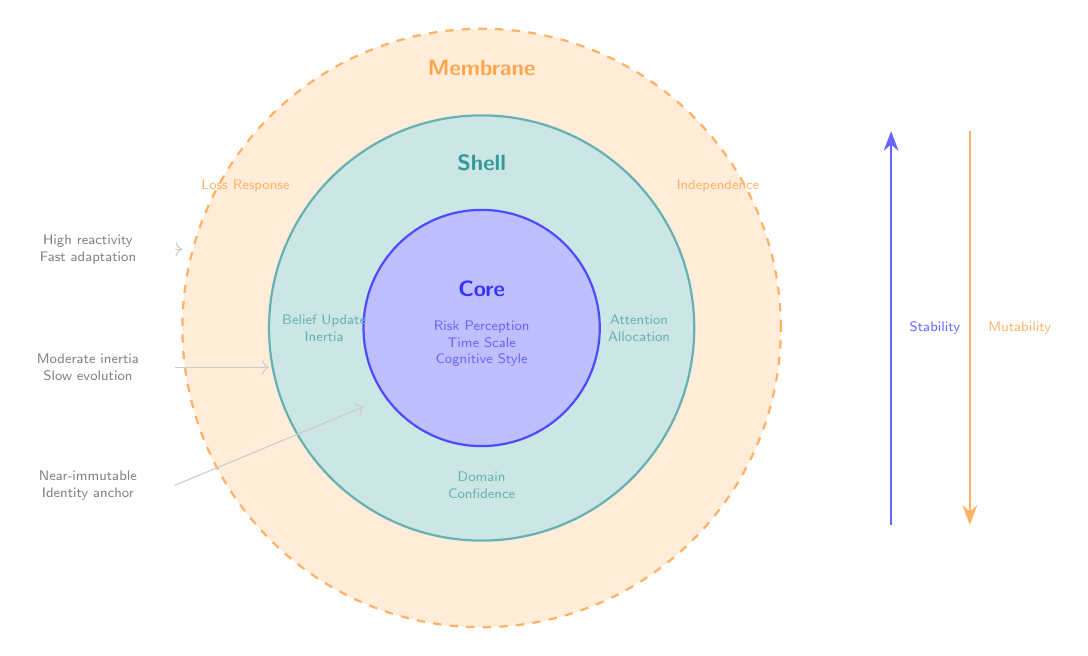
\begin{tikzpicture}[
    font=\sffamily\small
]

% Membrane (outermost)
\fill[orange!15] (0,0) circle (3.8cm);
\draw[orange!60, thick, dashed] (0,0) circle (3.8cm);

% Shell (middle)
\fill[teal!20] (0,0) circle (2.7cm);
\draw[teal!60, thick] (0,0) circle (2.7cm);

% Core (innermost)
\fill[blue!25] (0,0) circle (1.5cm);
\draw[blue!70, thick] (0,0) circle (1.5cm);

% Core labels
\node[font=\sffamily\footnotesize\bfseries, text=blue!80] at (0,0.5) {Core};
\node[font=\sffamily\tiny, text=blue!60, align=center] at (0,-0.2) {Risk Perception\\Time Scale\\Cognitive Style};

% Shell labels
\node[font=\sffamily\footnotesize\bfseries, text=teal!80] at (0,2.1) {Shell};
\node[font=\sffamily\tiny, text=teal!60, align=center] at (2.0,0) {Attention\\Allocation};
\node[font=\sffamily\tiny, text=teal!60, align=center] at (-2.0,0) {Belief Update\\Inertia};
\node[font=\sffamily\tiny, text=teal!60, align=center] at (0,-2.0) {Domain\\Confidence};

% Membrane labels
\node[font=\sffamily\footnotesize\bfseries, text=orange!70] at (0,3.3) {Membrane};
\node[font=\sffamily\tiny, text=orange!60] at (3.0,1.8) {Independence};
\node[font=\sffamily\tiny, text=orange!60] at (-3.0,1.8) {Loss Response};

% Right-side gradient arrows
\draw[-{Stealth[length=2.5mm]}, thick, blue!60]
    (5.2, -2.5) -- (5.2, 2.5)
    node[midway, right=3pt, font=\sffamily\tiny, text=blue!60, align=left] {Stability};

\draw[-{Stealth[length=2.5mm]}, thick, orange!60]
    (6.2, 2.5) -- (6.2, -2.5)
    node[midway, right=3pt, font=\sffamily\tiny, text=orange!60, align=left] {Mutability};

% Layer property annotations
\node[font=\sffamily\tiny, text=gray, align=center] at (-5.0, 1.0)
    {High reactivity\\Fast adaptation};
\node[font=\sffamily\tiny, text=gray, align=center] at (-5.0, -0.5)
    {Moderate inertia\\Slow evolution};
\node[font=\sffamily\tiny, text=gray, align=center] at (-5.0, -2.0)
    {Near-immutable\\Identity anchor};

\draw[gray!40, thin, ->] (-3.9, 1.0) -- (-3.8, 1.0);
\draw[gray!40, thin, ->] (-3.9, -0.5) -- (-2.7, -0.5);
\draw[gray!40, thin, ->] (-3.9, -2.0) -- (-1.5, -1.0);

\end{tikzpicture}
}
    \caption{Core-Shell-Membrane architecture of the \nous{} Schema. Inner layers are more stable; outer layers are more reactive. Arrows indicate the stability--mutability gradient.}
    \label{fig:csm}
\end{figure}

\begin{itemize}[leftmargin=*,itemsep=2pt]
    \item \textbf{Core} (near-immutable): Deep cognitive parameters that change rarely---risk perception, temporal orientation, and cognitive style. Analogous to personality traits shaped by culture and formative experience.
    \item \textbf{Shell} (slowly evolving): Domain-specialized parameters that adapt with sustained experience---attention allocation, belief update behavior, and domain-specific calibration. Requires many observations to shift.
    \item \textbf{Membrane} (reactive): Real-time behavioral signals---independence from crowd and loss response patterns. These fluctuate with recent experience but do not permanently alter the prior.
\end{itemize}

The design principle is: \emph{the deeper the layer, the higher the modification threshold and the slower the rate of change}---mirroring the observation that humans can change their mood in hours (membrane), revise a professional judgment over months (shell), but rarely alter their foundational risk attitudes (core)~\citep{tversky1992advances}.

\subsection{Eight Cognitive Dimensions}

Table~\ref{tab:dimensions} specifies the eight dimensions of the \nous{} Schema.

\begin{table}[t]
\centering
\caption{The eight dimensions of the \nous{} Schema. Each dimension includes parameter ranges, theoretical grounding, and minimum events required for extraction above population-prior confidence.}
\label{tab:dimensions}
\small
\begin{tabular}{@{}llllll@{}}
\toprule
\textbf{Dimension} & \textbf{Layer} & \textbf{Parameters} & \textbf{Range} & \textbf{Theory} & \textbf{Min.} \\
\midrule
Risk Perception & Core & $\alpha$, $\beta$, $\lambda$ & [0,1], [0,1], [1,5] & Prospect Theory~\citep{kahneman1979prospect} & 50 \\
Time Scale Pref. & Core & horizon\_bias, patience & [-1,1], [0,1] & Tetlock~\citep{tetlock2015superforecasting} & 20 \\
Cognitive Style & Core & analytical\_ratio, HF & [0,1], [-1,1] & System 1/2~\citep{kahneman2011thinking} & 30 \\
\midrule
Attention Alloc. & Shell & domain\_weights, blind\_spots & $\Delta^K$, list & Klein RPD~\citep{klein1998sources} & 20 \\
Belief Update & Shell & update\_rate, conf\_bias & [0,1], [0,1] & Griffiths~\citep{griffiths2008bayesian} & 30 \\
Domain Conf. & Shell & per-domain accuracy, freq. & [0,1], $\mathbb{N}$ & Klein--Kahneman~\citep{kahneman2009conditions} & 15 \\
\midrule
Independence & Membrane & contrarian, crowd\_sens. & [-1,1], [0,1] & Tetlock~\citep{tetlock2005expert} & 30 \\
Loss Response & Membrane & sunk\_cost, tilt, resilience & [0,1], [0,1], $\mathbb{R}^+$ & Damasio~\citep{damasio1994descartes} & 25 \\
\bottomrule
\end{tabular}
\end{table}

\subsection{Confidence Metadata and Graceful Degradation}

Each dimension carries confidence metadata: a composite score derived from data sufficiency (sigmoid function of event count relative to threshold), temporal stability (coefficient of variation across time windows), and internal consistency. When confidence falls below a threshold ($\tau = 0.2$), the dimension falls back to population priors from behavioral economics literature (\eg{} $\alpha = \beta = 0.88$, $\lambda = 2.25$ from \citealt{kahneman1979prospect}). This graceful degradation ensures that a \nous{} Instance is always well-defined, even for new users with sparse behavioral data.


% ============================================================
% 4. EXTRACTION PIPELINE
% ============================================================
\section{Extraction Pipeline}
\label{sec:extraction}

\subsection{Mathematical Foundation}
\label{sec:extraction:math}

We frame cognitive extraction as a Bayesian inverse inference problem. Let $H = \{(a_t, c_t, o_t)\}_{t=1}^T$ denote a user's behavioral history, where $a_t$ is an action (order, adjustment, view), $c_t$ is the decision context (market price, category, recent PnL), and $o_t$ is the observed outcome. Let $\theta = (\alpha, \beta, \lambda, h_{\text{bias}}, \ldots)$ denote the vector of cognitive parameters we wish to infer. The extraction problem is to compute the posterior:
\begin{equation}
    P(\theta \mid H) \propto P(H \mid \theta) \cdot P(\theta)
    \label{eq:bayes}
\end{equation}

The \emph{behavioral likelihood} $P(H \mid \theta)$ specifies the probability of observing behavior sequence $H$ given cognitive parameters $\theta$. For example, a user with high loss aversion ($\lambda \gg 2$) should exhibit longer holding durations on losing positions and faster profit-taking on winners; a user with low gain curvature ($\alpha \ll 1$) should show concave bet sizing as a function of probability. Each extractor implicitly defines a likelihood function over its input features.

The \emph{prior} $P(\theta)$ is grounded in the behavioral economics literature and corresponds directly to the population priors in our implementation: $\alpha = \beta = 0.88$, $\lambda = 2.25$~\citep{kahneman1979prospect}, neutral cognitive style, uniform attention, and moderate belief update rates. These priors ensure well-defined estimates even under data sparsity.

The \emph{posterior uncertainty} $P(\theta \mid H)$ naturally provides per-dimension confidence: dimensions with concentrated posteriors (many informative observations) receive high confidence, while dimensions with diffuse posteriors (sparse or noisy data) remain close to the prior. This is the theoretical basis for our confidence metadata and graceful degradation mechanism (Section~\ref{sec:priors}).

\paragraph{Relationship to current implementation.}
Our key methodological pivot relative to prior work formulating prediction markets as Bayesian inverse problems~\citep{madrigalcianci2026bayesian} is the inference target: rather than inferring event outcome parameters $\theta_{\text{event}}$ from market prices, we infer \emph{cognitive} parameters $\theta_{\text{cognitive}}$ from individual behavioral patterns. The current MVP implements this framework as \emph{point-estimate approximations}. For instance, the risk perception extractor's $\alpha$ fitting via \texttt{curve\_fit} is equivalent to a maximum a posteriori (MAP) estimate under an implicit Gaussian likelihood, but omits the full posterior distribution. The attention allocation extractor's exponential-decay weighted counts approximate the posterior mean of a Dirichlet-Multinomial model. These heuristic approximations are justified at the proof-of-concept stage: the parameter space is low-dimensional (17 scalar parameters across 8 dimensions), the behavioral signals are relatively direct (bet sizes, hold durations, category frequencies), and the primary goal is demonstrating that even approximate extraction produces meaningful cognitive differentiation upon injection.

Full Bayesian inference---via Markov chain Monte Carlo or variational methods---would provide three advantages left to future work: (1)~richer confidence estimates reflecting parameter covariance (\eg{} the correlation between $\alpha$ and $\lambda$), (2)~principled model comparison for extractor design, and (3)~sequential updating as new behavioral data arrives, naturally implementing the Core-Shell-Membrane stability gradient through appropriate prior strengths.

\subsection{Behavioral Event Schema}

The extraction pipeline operates on a stream of behavioral events from prediction market interactions. We define ten event types: \texttt{order} (buy/sell with price, amount, side, market category), \texttt{position\_close} (with PnL and hold duration), \texttt{adjustment} (position modification with price change context), \texttt{view} (market page view), \texttt{hesitation} (started but abandoned order), \texttt{cancel} (cancelled limit order), \texttt{comment}, \texttt{feed\_impression} (with click-through), \texttt{portfolio\_check}, and \texttt{resolution} (market outcome with Brier score).

\subsection{Feature Computation}

Raw events are transformed into typed feature vectors per user. A \texttt{UserFeatures} object aggregates all events by type, providing structured access to orders (with decision latency, order type), position closes (with PnL, hold duration), adjustments (with price change context and direction), and interaction signals (views, hesitations, feed impressions). This intermediate representation decouples event ingestion from dimension-specific extraction.

\subsection{Dimension Extraction Algorithms}

Eight stateless extractors operate on the feature vector, each returning dimension values plus confidence metadata (Algorithm~\ref{alg:pipeline}). We describe each briefly, with extended detail for risk perception.

\begin{algorithm}[t]
\caption{Nous Extraction Pipeline}
\label{alg:pipeline}
\KwIn{User ID $u$, Event Store $\mathcal{E}$}
\KwOut{NousInstance $\mathcal{N}_u$}

$\mathit{events} \gets \mathcal{E}.\mathtt{get\_events}(u)$\;
$\mathit{features} \gets \mathtt{compute\_features}(\mathit{events})$\;

\ForEach{extractor $e_i \in \{e_1, \ldots, e_8\}$}{
    $(\mathit{values}_i, \mathit{conf}_i) \gets e_i.\mathtt{extract}(\mathit{features})$\;
    \If{$\mathit{conf}_i < \tau$}{
        $\mathit{values}_i \gets \mathtt{POPULATION\_PRIORS}[i]$\;
        $\mathit{is\_prior}_i \gets \textbf{true}$\;
    }
}

$\mathcal{N}_u \gets \mathtt{NousInstance}(u,\ \mathit{values}_1, \ldots, \mathit{values}_8)$\;
\Return{$\mathcal{N}_u$}
\end{algorithm}

\paragraph{Risk Perception (Core).}
We fit the Prospect Theory value function~\citep{kahneman1979prospect}:
\begin{equation}
    v(x) = \begin{cases} x^\alpha & \text{if } x \geq 0 \text{ (gains)} \\ -\lambda(-x)^\beta & \text{if } x < 0 \text{ (losses)} \end{cases}
\end{equation}
The gain curvature $\alpha$ is estimated from the relationship between bet size and probability for YES-side orders (higher $\alpha$ = more linear, risk-neutral). We bin orders by probability deciles and fit $\hat{y} = x^\alpha$ via \texttt{scipy.optimize.curve\_fit}, with log-log regression as a fallback. The loss curvature $\beta$ is analogously estimated from NO-side orders. Loss aversion $\lambda$ is estimated from the asymmetry between winning and losing position behaviors, incorporating both PnL magnitude ratios and hold duration ratios (Algorithm~\ref{alg:risk}).

\begin{algorithm}[t]
\caption{Risk Perception via Prospect Theory}
\label{alg:risk}
\KwIn{Orders $\mathcal{O}$, Position Closes $\mathcal{C}$}
\KwOut{$\alpha, \beta, \lambda$}

$\mathcal{O}_{\text{YES}} \gets \{o \in \mathcal{O} \mid o.\mathit{side} = \text{YES} \land o.\mathit{price} > 0.1\}$\;
$\alpha \gets \texttt{fit\_curvature}(\{o.\mathit{price}\}, \{o.\mathit{amount}\}, \mathcal{O}_{\text{YES}})$ \tcp*{Binned power-law fit}

$\mathcal{O}_{\text{NO}} \gets \{o \in \mathcal{O} \mid o.\mathit{side} = \text{NO} \land o.\mathit{price} < 0.9\}$\;
$\beta \gets \texttt{fit\_curvature}(\{1 - o.\mathit{price}\}, \{o.\mathit{amount}\}, \mathcal{O}_{\text{NO}})$\;

$\mathcal{W} \gets \{c \in \mathcal{C} \mid c.\mathit{pnl} > 0\}$; $\mathcal{L} \gets \{c \in \mathcal{C} \mid c.\mathit{pnl} < 0\}$\;
$r_{\text{pnl}} \gets \overline{|\mathit{pnl}(\mathcal{L})|} \,/\, \overline{|\mathit{pnl}(\mathcal{W})|}$\;
$r_{\text{hold}} \gets \overline{\mathit{hold}(\mathcal{L})} \,/\, \overline{\mathit{hold}(\mathcal{W})}$\;
$\lambda \gets \text{clip}(1.0 + 0.5 \cdot r_{\text{pnl}} + 0.75 \cdot r_{\text{hold}},\ 1.0,\ 5.0)$\;

\Return{$\alpha, \beta, \lambda$}
\end{algorithm}

\paragraph{Attention Allocation (Shell).}
Domain weights are computed as weighted frequency counts with 30-day exponential decay: orders receive weight 3.0, views 1.0, hesitations 0.5, and clicked feed impressions 0.2. Blind spots are categories with attention weight below 2\% despite being available.

\paragraph{Cognitive Style (Core).}
The analytical ratio is a composite of four signals: median decision latency (longer $\to$ more analytical), bet size consistency (lower coefficient of variation $\to$ more analytical), limit-to-market order ratio, and cancellation frequency. The hedgehog-fox index is derived from the Herfindahl-Hirschman Index of category concentration: $\text{HFI} = 1 - 2 \cdot \frac{\text{HHI} - 1/n}{1 - 1/n}$.

\paragraph{Time Scale Preference (Core).}
Horizon bias compares the user's median holding duration to a market baseline (72h): $h = \text{clip}(2 \cdot \frac{\text{median\_hold}}{72} - 1,\ -1,\ 1)$. Patience index is the fraction of positions held past the user's own median.

\paragraph{Belief Update Inertia (Shell).}
Update rate measures the ratio of position adjustment magnitude to price change magnitude. Confirmation bias captures asymmetry: the ratio of mean confirming updates (increasing when price is favorable) to mean disconfirming updates.

\paragraph{Domain Confidence Map (Shell).}
Per-domain calibration computed as $1 - \overline{\text{Brier}}$ where $\text{Brier}(p, o) = (p - o)^2$, combined with relative bet sizing and entry frequency.

\paragraph{Independence Index (Membrane).}
Contrarian score measures how often the user bets against market consensus (price $>$ 0.5 $\Leftrightarrow$ market favors YES). Crowd sensitivity tracks adjustment frequency following large price moves ($>$10\%).

\paragraph{Loss Response (Membrane).}
Sunk cost sensitivity compares median hold durations for winning vs.\ losing positions. Tilt factor measures bet size variance in the hour after losses. Resilience half-life proxies recovery speed from portfolio check frequency patterns.

\subsection{Cold Start and Population Priors}

For users with insufficient behavioral data, each dimension falls back to population priors derived from the behavioral economics literature: $\alpha = \beta = 0.88$, $\lambda = 2.25$~\citep{kahneman1979prospect}; neutral cognitive style ($\text{analytical} = 0.5$, $\text{HFI} = 0$); uniform attention distribution; moderate belief update rate ($0.5$) with mild confirmation bias ($0.3$); and neutral independence. Confidence follows a sigmoid function of event count relative to dimension-specific thresholds (Table~\ref{tab:dimensions}).


% ============================================================
% 5. TRANSLATION AND INJECTION
% ============================================================
\section{Translation and Injection}
\label{sec:injection}

\subsection{Structure-to-Narrative Translation}

\paragraph{Translator v1: Threshold-based branching.}
The first-generation translator converts a parametric \nous{} Instance into natural-language cognitive instructions using discrete threshold-based branching. For each of seven dimensions, 2--3 parameter thresholds select among qualitative descriptions anchored in experiential language. For example, a low gain curvature ($\alpha < 0.55$) produces: ``Your marginal sensitivity to gains diminishes rapidly---going from a 10\% to a 20\% return barely doubles your excitement.'' This narrative anchoring strategy is motivated by the observation that LLMs respond more consistently to qualitative cognitive framing than to numerical parameter specifications~\citep{wei2022chain}. However, v1 suffers from an \emph{information bottleneck}: continuous parameters are quantized into 2--3 discrete buckets, discarding the fine-grained individual variation that the extraction pipeline captures.

\paragraph{Translator v2: Continuous parameterization.}
The second-generation translator eliminates discrete bucketing in favor of five design principles: (1)~\emph{Continuous parameter embedding}---exact numerical values are presented alongside population-relative positioning (z-scores and $n$-times-mean ratios), preserving the full information content of extracted parameters. (2)~\emph{Behavioral inference chains}---each parameter value triggers a chain of behavioral consequences (``A \$100 loss feels equivalent to missing a \$350 gain $\to$ you need at least 3.5:1 reward/risk $\to$ your first instinct in downturns is to protect existing positions''). (3)~\emph{Cross-dimension interaction effects}---the translator identifies and explicitly describes emergent behaviors from parameter combinations (\eg{} high loss aversion + long horizon $\to$ gravitates toward ``can't go to zero'' assets). (4)~\emph{Contrastive anchoring}---the prompt opens with the three largest deviations from the population mean, immediately establishing how this mind differs from the average. (5)~\emph{Behavioral exemplars}---concrete past-decision vignettes generated from the cognitive parameters, leveraging in-context pattern induction. In multi-model experiments (Section~\ref{sec:experiments}), v2 achieves a +16.3\% mean trigram diversity improvement over v1 across three models, matching handwritten persona baselines on textual diversity while remaining fully automated (see Appendix~\ref{app:translator} for a complete v2 output example).

\subsection{Intensity Parameter}

An intensity parameter $\iota \in [0, 1]$ controls injection strength:
\begin{itemize}[leftmargin=*,itemsep=1pt]
    \item $\iota < 0.3$: ``Cognitive tendencies for reference''---light suggestions.
    \item $0.3 \leq \iota \leq 0.7$: ``Your cognitive characteristics''---moderate framing.
    \item $\iota > 0.7$: ``Your cognitive substrate (mandatory)''---strong directive that these traits are the agent's cognitive reality.
\end{itemize}
At low intensity, only the top 3 dimensions by confidence are included, reducing prompt length while preserving the most distinctive characteristics.

\subsection{Prompt Assembly}

The injection mechanism places \nous{} instructions \emph{first} in the system prompt, before role specification:

\begin{equation*}
    \texttt{system\_prompt} = \underbrace{\texttt{nous\_instructions}}_{\text{cognitive foundation}} + \underbrace{\texttt{role\_prompt}}_{\text{task specification}}
\end{equation*}

This ordering reflects the architectural thesis: cognitive priors are the foundation upon which role-specific behavior is built, not an afterthought appended to existing prompts (Figure~\ref{fig:architecture}).

\begin{figure}[t]
    \centering
    \resizebox{0.55\textwidth}{!}{% Figure: Agent Architecture — Nous as cognitive preprocessing layer
% Information flow: Input → φ (Nous) → r (Foundation Model) → Output
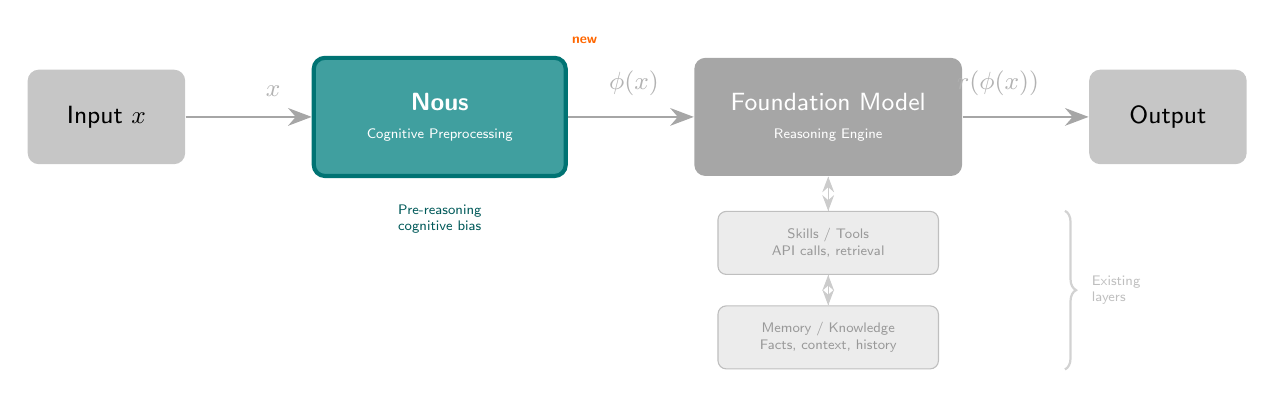
\begin{tikzpicture}[
    node distance=1.8cm,
    block/.style={
        rectangle, rounded corners=4pt,
        minimum height=1.2cm, text=white,
        font=\sffamily\small, draw=none, align=center
    },
    aux/.style={
        rectangle, rounded corners=3pt,
        minimum width=2.4cm, minimum height=0.8cm,
        font=\sffamily\tiny, align=center,
        draw=gray!50, fill=gray!15, text=gray!80
    },
    mainflow/.style={-{Stealth[length=3mm]}, thick, gray!70},
    auxflow/.style={-{Stealth[length=2mm]}, thin, gray!40},
    mathlabel/.style={font=\small, text=gray!60},
    label/.style={font=\sffamily\tiny, text=gray!60}
]

% === Main flow (left to right) ===

% Input
\node[block, fill=gray!45, text=black, minimum width=2cm] (input) at (0,0)
    {Input $x$};

% Nous — highlighted
\node[block, fill=teal!75, minimum width=3.2cm, minimum height=1.5cm,
      line width=1.5pt, draw=teal!90!black,
      font=\sffamily\small\bfseries, right=1.6cm of input] (nous)
    {\nous{}\\[-1pt]{\normalfont\sffamily\tiny Cognitive Preprocessing}};
\node[font=\sffamily\tiny\bfseries, text=orange!80!red, anchor=south west]
    at ([xshift=-2pt, yshift=1pt]nous.north east) {\textsc{new}};

% Foundation Model
\node[block, fill=gray!70, minimum width=3.4cm, minimum height=1.5cm,
      right=1.6cm of nous] (model)
    {Foundation Model\\[-1pt]{\normalfont\sffamily\tiny Reasoning Engine}};

% Output
\node[block, fill=gray!45, text=black, minimum width=2cm,
      right=1.6cm of model] (output)
    {Output};

% Main flow arrows
\draw[mainflow] (input) -- (nous);
\draw[mainflow] (nous) -- (model);
\draw[mainflow] (model) -- (output);

% Math labels along arrows
\node[mathlabel, above=4pt] at ($(input)!0.5!(nous)$) {$x$};
\node[mathlabel, above=4pt] at ($(nous)!0.5!(model)$) {$\phi(x)$};
\node[mathlabel, above=4pt] at ($(model)!0.5!(output)$) {$r(\phi(x))$};

% === Auxiliary modules (below Foundation Model) ===

\node[aux, minimum width=2.8cm] (skills) at ($(model) + (0, -1.6)$)
    {Skills / Tools\\{\tiny API calls, retrieval}};

\node[aux, minimum width=2.8cm] (memory) at ($(model) + (0, -2.8)$)
    {Memory / Knowledge\\{\tiny Facts, context, history}};

% Auxiliary arrows (bidirectional)
\draw[auxflow] (model.south) -- (skills.north);
\draw[auxflow] (skills.north) -- (model.south);
\draw[auxflow] (skills.south) -- (memory.north);
\draw[auxflow] (memory.north) -- (skills.south);

% Brace for auxiliary
\draw[decorate, decoration={brace, amplitude=4pt}, thick, gray!35]
    ([xshift=1.6cm]skills.north east) -- ([xshift=1.6cm]memory.south east)
    node[midway, right=6pt, font=\sffamily\tiny, text=gray!50, align=left]
    {Existing\\layers};

% Annotation: what Nous does
\node[label, text=teal!70!black, align=center, anchor=north]
    at ([yshift=-6pt]nous.south)
    {Pre-reasoning\\cognitive bias};

\end{tikzpicture}
}
    \caption{Agent architecture with \nous{} as a cognitive preprocessing layer. Information passes through the \nous{} prior $\phi$ before entering the foundation model's reasoning pipeline $r$, implementing $\text{output} = r(\phi(x))$.}
    \label{fig:architecture}
\end{figure}

\subsection{Beyond Prompt Injection: A Spectrum of Methods}
\label{sec:injection:spectrum}

System prompt injection is the shallowest point on a spectrum of possible injection methods, ordered by the depth at which they intervene in the model's computation:

\begin{table}[h]
\centering
\small
\begin{tabular}{@{}llllc@{}}
\toprule
\textbf{Depth} & \textbf{Method} & \textbf{Acts On} & \textbf{Requirements} & \textbf{Avail.} \\
\midrule
Shallow & System prompt (this work) & Text instruction & Any API & \checkmark \\
Med-shallow & Few-shot exemplars & In-context learning & Any API & \checkmark \\
Medium & Logit bias / decoding & Token sampling & logit\_bias API & Partial \\
Med-deep & Soft prompt / prefix tuning & Embedding space & Model weights & Open-src \\
Deep & LoRA adapter per-\nous{} & Weight subspace & Weights + training & Feasible \\
Deepest & Activation steering & Internal activations & Weights + interp. & Research \\
\bottomrule
\end{tabular}
\end{table}

The fundamental limitation of system prompt injection is that cognitive priors should act \emph{before} reasoning, yet the prompt enters the same processing pipeline as the user query. Instructing a model to ``perceive risk differently'' requires the instruction itself to be processed through the model's existing (mean-field) cognitive substrate---the very substrate we seek to override.

\emph{Activation steering}~\citep{zou2023representation, turner2024activation} represents the theoretically optimal injection point: directly adding direction vectors to the model's intermediate representations, bypassing the text-layer bottleneck entirely. Recent work has demonstrated that interpretable ``concept directions'' exist in activation space for attributes such as honesty, risk tolerance, and analytical depth---precisely the dimensions in the \nous{} Schema.

\emph{Few-shot exemplar injection} is the most promising near-term upgrade. Rather than abstractly describing a cognitive style, one provides concrete examples of how the source human made past decisions. This leverages the LLM's strongest capability (in-context pattern induction) rather than its weakest (following abstract meta-cognitive instructions). The \nous{} Schema is compatible with this approach: extracted parameters can be used to retrieve or generate representative decision vignettes.

We chose system prompt injection for the current implementation because it is model-agnostic, zero-cost, and immediately deployable. Critically, the \nous{} Schema is designed as a \emph{representation standard independent of injection method}---the same \nous{} Instance can be injected via prompts today and via activation steering tomorrow, without modifying the extraction pipeline or the schema itself.


% ============================================================
% 6. EXPERIMENTS
% ============================================================
\section{Experiments}
\label{sec:experiments}

\subsection{Experimental Design}

We conduct a proof-of-concept experiment to evaluate whether \nous{} injection produces genuine cognitive differentiation in LLM outputs. The design involves:

\paragraph{Personas.} Three synthetic personas spanning the cognitive parameter space:
\begin{itemize}[leftmargin=*,itemsep=1pt]
    \item \textbf{Conservative Veteran}: moderate gain curvature ($\alpha = 0.65$), high loss aversion ($\lambda = 3.5$), long-term focus ($h_{\text{bias}} = 0.6$), analytical ($\text{AR} = 0.8$), hedgehog-leaning ($\text{HFI} = -0.5$), concentrated attention on politics (30\%) and business (25\%).
    \item \textbf{Aggressive Tech Optimist}: near-linear gain sensitivity ($\alpha = 0.95$), low loss aversion ($\lambda = 1.5$), short-term focus ($h_{\text{bias}} = -0.5$), intuitive ($\text{AR} = 0.3$), strong hedgehog ($\text{HFI} = -0.7$), concentrated attention on tech (35\%) and crypto (30\%).
    \item \textbf{Balanced Analyst}: population-mean parameters ($\alpha = 0.88$, $\lambda = 2.25$), fox-like integration ($\text{HFI} = 0.6$), uniformly distributed attention across domains.
\end{itemize}
Each persona generates 800 synthetic behavioral events, from which \nous{} Instances are extracted via the full pipeline. A \textbf{Control} agent receives the base role prompt without any cognitive prior injection.

\paragraph{Test Questions.} Five scenarios designed to probe different cognitive dimensions:
\begin{enumerate}[leftmargin=*,itemsep=1pt]
    \item \textbf{BTC Investment}: BTC at \$85K with conflicting whale sell-off and ETF inflow signals.
    \item \textbf{AI Startup Risk}: \$500M valuation, GPT-5-level tech, \$8M/month burn, no revenue.
    \item \textbf{Ambiguous Signal}: Government official wallet buying DeFi tokens---insider trading or coincidence?
    \item \textbf{Domain Preference}: ``List three trends worth watching today and explain why.''
    \item \textbf{DeFi Time Preference}: Fast MVP launch vs.\ three-month security audit.
\end{enumerate}

\paragraph{Models and Conditions.} We evaluate three open-weight models spanning different architectures and scales: Qwen3-32B, DeepSeek-R1-32B, and Llama~3.1-8B, all served locally via Ollama with temperature 0.7 and injection intensity 0.8. Each model is tested under four conditions: (1)~\emph{Nous~v2}---cognitive priors translated by the continuous v2 translator; (2)~\emph{Nous~v1}---the same priors translated by the threshold-based v1 translator; (3)~\emph{Handwritten}---manually authored persona descriptions with equivalent information content (\eg{} ``You are a conservative, risk-averse analyst who focuses on downside protection and long-term structural trends''); and (4)~\emph{Control}---the base role prompt without any cognitive prior injection. Each condition is run 3 times per question for a total of approximately 450 LLM calls across the full experimental matrix. Cross-language experiments (Chinese vs.\ English) use the v1 translator on Qwen3-32B.

\subsection{Qualitative Results}

Table~\ref{tab:results} summarizes the qualitative differentiation observed across all five questions.

\begin{table}[t]
\centering
\caption{Qualitative differentiation across five test scenarios. Stars indicate the degree of judgment-level (not merely stylistic) differentiation observed.}
\label{tab:results}
\footnotesize
\setlength{\tabcolsep}{3.5pt}
\newcommand{\rp}{\raggedright\arraybackslash}
\begin{tabular}{@{}>{\rp}p{1.9cm}>{\rp}p{2.2cm}>{\rp}p{2.5cm}>{\rp}p{2.2cm}>{\rp}p{1.7cm}c@{}}
\toprule
\textbf{Question} & \textbf{Conservative} & \textbf{Aggressive} & \textbf{Balanced} & \textbf{Control} & \textbf{Diff.} \\
\midrule
Q1: BTC & Hedge, reduce exposure, contagion risk & Grid buy, ETF support, 68\% recovery & Multi-hypothesis, structural pressure & Bearish, \$75--78K & $\star\star\star\star\star$ \\
\addlinespace
Q2: AI Risk & Reject (loss aversion dominates) & Deconstruct investment conditions & Structured rejection, valuation analysis & Reject & $\star\star\star\star$ \\
\addlinespace
Q3: Signal & Avoid, wait for confirmation & Reverse-deduce, 65--75\% insider & Multi-hypothesis verification & Quanti\-tative analysis & $\star\star\star\star$ \\
\addlinespace
Q4: Domain & Fusion energy, mfg.\ AI, geopolitics & Quantum computing, gene editing, sovereign crypto & BTC halving, mining cycle & AI medicine, climate eng. & $\star\star\star\star\star$ \\
\addlinespace
Q5: DeFi & Security audit (B) & Security audit (B) & Security audit (B) & Security audit (B) & $\star$ \\
\bottomrule
\end{tabular}
\end{table}

\textbf{Q1 (BTC Investment)} produced the strongest differentiation. The Conservative agent focused on whale contagion effects and recommended position reduction. The Aggressive agent reframed the dip as an opportunity, proposing a grid-buy strategy from \$82K downward and citing a ``68\% historical recovery probability.'' The Balanced agent maintained multiple hypotheses simultaneously.

\textbf{Q4 (Domain Preference)} demonstrated that attention allocation is the most directly attributable injection dimension. Each agent selected completely different topic domains: the Conservative chose geopolitical and energy topics, the Aggressive chose quantum computing and biotech, and the Balanced focused on BTC market structure---directly reflecting their injected attention weights.

\textbf{Q5 (DeFi Time Preference)} revealed an important boundary: all four agents (including Control) chose the security audit option. The LLM's safety-aligned training overrode the Aggressive persona's injected time preference. We discuss this ``correct answer bias'' in Section~\ref{sec:discussion}.

\subsection{Translator Comparison and Baseline Results}

We compute trigram Jaccard distance as a lightweight textual diversity proxy: $d(A, B) = 1 - |T_A \cap T_B| / |T_A \cup T_B|$, where $T_X$ is the set of character trigrams in response $X$. Intra-method diversity measures the mean pairwise distance between the three personas within each injection condition. Table~\ref{tab:v2results} reports results across all three models and four conditions.

\begin{table}[t]
\centering
\caption{Trigram Jaccard diversity (intra-method, mean pairwise) by model and injection condition. Higher values indicate greater textual differentiation between personas. Mean v2 improvement over v1: +16.3\%.}
\label{tab:v2results}
\small
\begin{tabular}{@{}lcccrr@{}}
\toprule
\textbf{Model} & \textbf{Nous v2} & \textbf{Nous v1} & \textbf{Handwritten} & \textbf{v2 vs.\ v1} & \textbf{v2 vs.\ HW} \\
\midrule
Llama 3.1-8B & 0.629 & 0.610 & 0.627 & +3.1\% & +0.3\% \\
Qwen3-32B & 0.575 & 0.373 & 0.381 & +54.3\% & +50.9\% \\
DeepSeek-R1-32B & 0.666 & 0.625 & 0.687 & +6.6\% & $-$3.1\% \\
\midrule
\textbf{Mean} & \textbf{0.623} & \textbf{0.536} & \textbf{0.565} & \textbf{+16.3\%} & \textbf{+10.3\%} \\
\bottomrule
\end{tabular}
\end{table}

Three findings emerge from the multi-model comparison:

\begin{enumerate}[leftmargin=*,itemsep=2pt]
    \item \textbf{v2 $>$ v1 consistently.} The v2 translator produces higher trigram diversity than v1 on all three models (+3.1\% to +54.3\%), with the largest gain on Qwen3-32B where v1 diversity was particularly low (0.373). The continuous parameterization and behavioral inference chains of v2 resolve the information bottleneck that limited v1.
    \item \textbf{v2 $\approx$ handwritten baselines.} Nous v2 matches or exceeds handwritten persona diversity on 2 of 3 models. On DeepSeek-R1-32B, handwritten personas achieve slightly higher diversity (0.687 vs.\ 0.666), suggesting that model-specific prompt sensitivity remains a factor. The mean advantage of v2 over handwritten (+10.3\%) is driven primarily by Qwen3-32B.
    \item \textbf{Path diversity $>$ conclusion diversity.} Per-question analysis reveals that reasoning-path questions produce higher diversity than conclusion-oriented questions, consistent with the ``correct answer bias'' observed qualitatively.\footnote{Per-question mean trigram diversity (v2, cross-model): investment 0.604, risk assessment 0.665, ambiguous signal 0.600, time preference 0.583, domain preference 0.664. Source: \texttt{results\_v2\_full/cross\_model\_summary.json}.} The exception is domain preference, where attention allocation injection directly determines topic selection.
\end{enumerate}

\subsection{Cross-Language Comparison}

Table~\ref{tab:crosslang} compares Chinese and English injection results using the v1 translator on Qwen3-32B. Cross-language experiments with the v2 translator are left to future work.

\begin{table}[t]
\centering
\caption{Cross-language comparison of injection effectiveness. English injection achieves deeper cognitive penetration despite lower raw trigram diversity (Chinese trigrams have inherently low overlap).}
\label{tab:crosslang}
\small
\begin{tabular}{@{}lccl@{}}
\toprule
\textbf{Metric} & \textbf{Chinese} & \textbf{English} & \textbf{Interpretation} \\
\midrule
Mean Nous inter-diversity & 0.949 & 0.812 & Chinese near random baseline \\
Mean distance from control & 0.950 & 0.753 & English more interpretable \\
\addlinespace
Q2 Aggressive judgment & Reject & Conditional Yes & English penetrates deeper \\
Q3 Aggressive specificity & ``Likely insider'' & ``65--75\%, 30--40\% capital'' & English: concrete actions \\
Q5 consensus override & All choose B & All choose B & Cross-language consistent \\
\bottomrule
\end{tabular}
\end{table}

The most striking finding is the Aggressive persona's divergent judgment on Q2 (AI startup): in Chinese, all agents (including Aggressive) rejected the investment, but in English, the Aggressive agent produced a ``Conditional Yes with Caveats''---the first instance where a persona's judgment \emph{direction} differed. This suggests that English injection achieves deeper cognitive penetration, possibly because the model (Qwen3-32B) has stronger instruction-following in English, or because Chinese safety training produces more conservative outputs.

The high Chinese trigram diversity (0.949) is largely a measurement artifact: Chinese character trigrams have inherently lower overlap than English word trigrams, pushing the metric toward the random baseline regardless of semantic content. The English diversity score (0.812) is more informative for assessing genuine cognitive differentiation.

\paragraph{Linguistic asymmetry in pre-training and alignment.}
The observed cross-language injection asymmetry likely reflects structural differences in how Qwen3-32B processes Chinese versus English inputs. First, pre-training data composition: while Qwen3 is trained on a multilingual corpus with substantial Chinese representation, its instruction-following capabilities may be disproportionately tuned on English data, as most open-source instruction-tuning datasets (OpenAssistant, Alpaca, ShareGPT) are predominantly English. Second, safety alignment intensity: Chinese-language safety training may impose stronger conservatism constraints, as Chinese AI regulation emphasizes ``positive and healthy'' outputs more explicitly than Western alignment frameworks. This could explain why the Aggressive persona's ``Conditional Yes'' on Q2 emerged only in English---the Chinese safety layer effectively imposed an additional barrier against risk-tolerant outputs.

These observations have practical implications for \nous{} deployment: For Qwen3-32B, the translator benefits from defaulting to English for cognitive injection, using a separate language-control instruction to set the response language. Whether this advantage extends to other models---particularly those with stronger non-English instruction-following---requires further investigation.

\subsection{Key Findings}

\begin{enumerate}[leftmargin=*,itemsep=2pt]
    \item \textbf{4/5 judgment-level differentiation}: Injection produces cognitive divergence, not mere stylistic variation, on tasks without clear ``correct answers.''
    \item \textbf{Cognitive, not stylistic}: Differences reflect distinct risk attitudes, attention priorities, and decision frameworks---not just vocabulary or tone.
    \item \textbf{Attention allocation most directly attributable}: Q4 (domain preference) shows near-perfect mapping from injected weights to selected topics.
    \item \textbf{Cross-model robustness}: The general differentiation pattern (4/5 tasks showing judgment-level variation) is observed across all three models, though with varying intensity. Per-model quantitative results are reported in Table~\ref{tab:v2results}; detailed per-model qualitative analysis is left to future work.
    \item \textbf{v2 resolves the information bottleneck}: The continuous v2 translator achieves +16.3\% mean \emph{textual} diversity improvement over v1, with the largest gain (+54.3\%) on the model where v1 was most constrained (Qwen3-32B). Whether this textual diversity gain corresponds to proportional gains in semantic or inferential diversity remains to be verified with richer metrics.
    \item \textbf{Automated $\approx$ handwritten on textual diversity}: Nous v2 matches handwritten persona baselines on trigram diversity (+10.3\% mean), suggesting that structured extraction and translation can replace manual persona authoring for generating diverse reasoning paths. However, handwritten personas retain an advantage on structured-output diversity (Limitation~7), indicating that conclusion-level differentiation requires further translator improvement.
    \item \textbf{Preliminary observation---path vs.\ conclusion diversity}: In our five-question test set, questions requiring extended reasoning paths (investment, risk assessment, ambiguous signal) produced higher inter-persona diversity than the single conclusion-oriented question (time preference), though this observation is based on too few conclusion-oriented questions ($n=1$) to be conclusive.
    \item \textbf{Correct answer bias}: When a question has a socially consensual answer (Q5: security audit), LLM alignment overrides the injected prior.
    \item \textbf{English $>$ Chinese injection depth}: English prompts achieve deeper cognitive penetration on Qwen3-32B (v1 translator). Control agents default to ``cautious analyst'' behavior across all models.
\end{enumerate}


% ============================================================
% RESULTS FIGURE
% ============================================================
\begin{figure}[t]
    \centering
    \resizebox{0.85\textwidth}{!}{% Figure 4: Experiment Results — Differentiation Heatmap
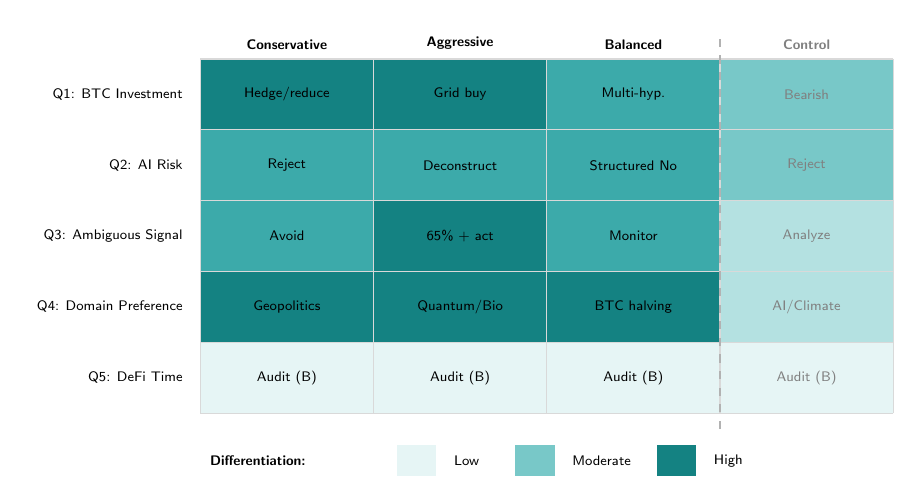
\begin{tikzpicture}[
    font=\sffamily\tiny
]

% Define color scale: low differentiation = light, high = dark teal
\definecolor{diff1}{RGB}{230, 245, 245}  % very low
\definecolor{diff2}{RGB}{180, 225, 225}  % low
\definecolor{diff3}{RGB}{120, 200, 200}  % moderate
\definecolor{diff4}{RGB}{60, 170, 170}   % high
\definecolor{diff5}{RGB}{20, 130, 130}   % very high

% Grid dimensions
\def\cellw{2.2cm}
\def\cellh{0.9cm}

% Column headers (agents)
\node[anchor=south, font=\sffamily\tiny\bfseries] at (1.1, 4.5) {Conservative};
\node[anchor=south, font=\sffamily\tiny\bfseries] at (3.3, 4.5) {Aggressive};
\node[anchor=south, font=\sffamily\tiny\bfseries] at (5.5, 4.5) {Balanced};
\node[anchor=south, font=\sffamily\tiny\bfseries, text=gray] at (7.7, 4.5) {Control};

% Row labels (questions)
\node[anchor=east, font=\sffamily\tiny] at (-0.1, 3.6+0.45) {Q1: BTC Investment};
\node[anchor=east, font=\sffamily\tiny] at (-0.1, 2.7+0.45) {Q2: AI Risk};
\node[anchor=east, font=\sffamily\tiny] at (-0.1, 1.8+0.45) {Q3: Ambiguous Signal};
\node[anchor=east, font=\sffamily\tiny] at (-0.1, 0.9+0.45) {Q4: Domain Preference};
\node[anchor=east, font=\sffamily\tiny] at (-0.1, 0+0.45) {Q5: DeFi Time};

% Q1 row — high differentiation
\fill[diff5] (0, 3.6) rectangle +(\cellw, \cellh);
\fill[diff5] (2.2, 3.6) rectangle +(\cellw, \cellh);
\fill[diff4] (4.4, 3.6) rectangle +(\cellw, \cellh);
\fill[diff3] (6.6, 3.6) rectangle +(\cellw, \cellh);

% Q2 row
\fill[diff4] (0, 2.7) rectangle +(\cellw, \cellh);
\fill[diff4] (2.2, 2.7) rectangle +(\cellw, \cellh);
\fill[diff4] (4.4, 2.7) rectangle +(\cellw, \cellh);
\fill[diff3] (6.6, 2.7) rectangle +(\cellw, \cellh);

% Q3 row
\fill[diff4] (0, 1.8) rectangle +(\cellw, \cellh);
\fill[diff5] (2.2, 1.8) rectangle +(\cellw, \cellh);
\fill[diff4] (4.4, 1.8) rectangle +(\cellw, \cellh);
\fill[diff2] (6.6, 1.8) rectangle +(\cellw, \cellh);

% Q4 row — highest differentiation
\fill[diff5] (0, 0.9) rectangle +(\cellw, \cellh);
\fill[diff5] (2.2, 0.9) rectangle +(\cellw, \cellh);
\fill[diff5] (4.4, 0.9) rectangle +(\cellw, \cellh);
\fill[diff2] (6.6, 0.9) rectangle +(\cellw, \cellh);

% Q5 row — low differentiation
\fill[diff1] (0, 0) rectangle +(\cellw, \cellh);
\fill[diff1] (2.2, 0) rectangle +(\cellw, \cellh);
\fill[diff1] (4.4, 0) rectangle +(\cellw, \cellh);
\fill[diff1] (6.6, 0) rectangle +(\cellw, \cellh);

% Cell labels — brief behavioral descriptions
\node at (1.1, 4.05) {Hedge/reduce};
\node at (3.3, 4.05) {Grid buy};
\node at (5.5, 4.05) {Multi-hyp.};
\node[text=gray] at (7.7, 4.05) {Bearish};

\node at (1.1, 3.15) {Reject};
\node at (3.3, 3.15) {Deconstruct};
\node at (5.5, 3.15) {Structured No};
\node[text=gray] at (7.7, 3.15) {Reject};

\node at (1.1, 2.25) {Avoid};
\node at (3.3, 2.25) {65\% + act};
\node at (5.5, 2.25) {Monitor};
\node[text=gray] at (7.7, 2.25) {Analyze};

\node at (1.1, 1.35) {Geopolitics};
\node at (3.3, 1.35) {Quantum/Bio};
\node at (5.5, 1.35) {BTC halving};
\node[text=gray] at (7.7, 1.35) {AI/Climate};

\node at (1.1, 0.45) {Audit (B)};
\node at (3.3, 0.45) {Audit (B)};
\node at (5.5, 0.45) {Audit (B)};
\node[text=gray] at (7.7, 0.45) {Audit (B)};

% Grid lines
\foreach \y in {0, 0.9, 1.8, 2.7, 3.6, 4.5} {
    \draw[gray!30] (0, \y) -- (8.8, \y);
}
\foreach \x in {0, 2.2, 4.4, 6.6, 8.8} {
    \draw[gray!30] (\x, 0) -- (\x, 4.5);
}

% Dashed line separating Nous agents from Control
\draw[dashed, gray!60, thick] (6.6, -0.2) -- (6.6, 4.8);

% Legend
\node[anchor=west, font=\sffamily\tiny\bfseries] at (0, -0.6) {Differentiation:};
\fill[diff1] (2.5, -0.8) rectangle (3.0, -0.4);
\node[anchor=west] at (3.1, -0.6) {Low};
\fill[diff3] (4.0, -0.8) rectangle (4.5, -0.4);
\node[anchor=west] at (4.6, -0.6) {Moderate};
\fill[diff5] (5.8, -0.8) rectangle (6.3, -0.4);
\node[anchor=west] at (6.4, -0.6) {High};

\end{tikzpicture}
}
    \caption{Differentiation heatmap across five test scenarios and four agents. Color intensity indicates the degree of judgment-level divergence from other agents. The dashed line separates \nous{}-injected agents from the Control. Q4 (Domain Preference) shows the most clearly dimension-attributable differentiation; Q5 (DeFi Time) shows uniform convergence due to correct answer bias.}
    \label{fig:results}
\end{figure}


% ============================================================
% PIPELINE FIGURE
% ============================================================
\begin{figure}[t]
    \centering
    \resizebox{\textwidth}{!}{% Figure: Extraction and Injection Pipeline
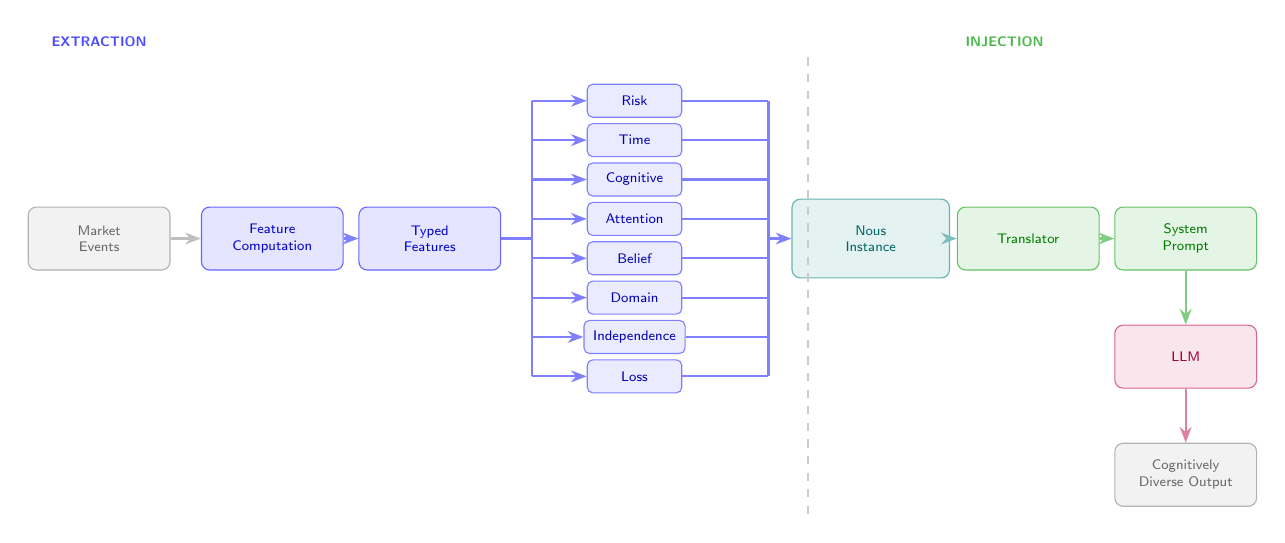
\begin{tikzpicture}[
    node distance=1.2cm and 1.6cm,
    box/.style={rectangle, rounded corners=3pt, draw=#1!60, fill=#1!10,
                minimum height=0.8cm, minimum width=1.8cm,
                font=\sffamily\tiny, align=center, text=#1!80!black},
    smallbox/.style={rectangle, rounded corners=2pt, draw=#1!50, fill=#1!8,
                minimum height=0.42cm, minimum width=1.2cm,
                font=\sffamily\tiny, align=center, text=#1!70!black},
    arr/.style={-{Stealth[length=2mm]}, thick, #1!50},
    bus/.style={thick, #1!50},
    phase/.style={font=\sffamily\tiny\bfseries, text=#1!70},
]

% Phase labels
\node[phase=blue] at (0, 2.5) {EXTRACTION};
\node[phase=green!60!black] at (11.5, 2.5) {INJECTION};

% Source
\node[box=gray] (events) at (0, 0) {Market\\Events};

% Event Parser
\node[box=blue] (parser) at (2.2, 0) {Feature\\Computation};

% Features
\node[box=blue] (features) at (4.2, 0) {Typed\\Features};

% Extractors (single column)
\node[smallbox=blue] (e1) at (6.8,  1.75) {Risk};
\node[smallbox=blue] (e2) at (6.8,  1.25) {Time};
\node[smallbox=blue] (e3) at (6.8,  0.75) {Cognitive};
\node[smallbox=blue] (e4) at (6.8,  0.25) {Attention};
\node[smallbox=blue] (e5) at (6.8, -0.25) {Belief};
\node[smallbox=blue] (e6) at (6.8, -0.75) {Domain};
\node[smallbox=blue] (e7) at (6.8, -1.25) {Independence};
\node[smallbox=blue] (e8) at (6.8, -1.75) {Loss};

% Nous Instance
\node[box=teal, minimum width=2.0cm, minimum height=1.0cm] (nous) at (9.8, 0) {Nous\\Instance};

% Translator
\node[box=green!60!black] (trans) at (11.8, 0) {Translator};

% System Prompt
\node[box=green!60!black] (prompt) at (13.8, 0) {System\\Prompt};

% LLM
\node[box=purple] (llm) at (13.8, -1.5) {LLM};

% Output
\node[box=gray] (output) at (13.8, -3.0) {Cognitively\\Diverse Output};

% === Arrows — extraction phase ===
\draw[arr=gray] (events) -- (parser);
\draw[arr=blue] (parser) -- (features);

% Fan-out: features → vertical bus → each extractor
\coordinate (fork) at (5.5, 0);
\draw[bus=blue] (features.east) -- (fork);
\draw[bus=blue] (fork |- e1.west) -- (fork |- e8.west);
\foreach \e in {e1,e2,e3,e4,e5,e6,e7,e8} {
    \draw[arr=blue] (fork |- \e.west) -- (\e.west);
}

% Fan-in: each extractor → vertical bus → Nous
\coordinate (merge) at (8.5, 0);
\foreach \e in {e1,e2,e3,e4,e5,e6,e7,e8} {
    \draw[bus=blue] (\e.east) -- (merge |- \e.east);
}
\draw[bus=blue] (merge |- e1.east) -- (merge |- e8.east);
\draw[arr=blue] (merge) -- (nous.west);

% === Arrows — injection phase ===
\draw[arr=teal] (nous) -- (trans);
\draw[arr=green!60!black] (trans) -- (prompt);
\draw[arr=green!60!black] (prompt) -- (llm);
\draw[arr=purple] (llm) -- (output);

% Dashed separation line
\draw[dashed, gray!40, thick] (9.0, 2.3) -- (9.0, -3.5);

\end{tikzpicture}
}
    \caption{End-to-end extraction and injection pipeline. Blue nodes represent the extraction phase (behavioral events $\to$ features $\to$ 8 parallel extractors $\to$ \nous{} Instance); green nodes represent the injection phase (translator $\to$ system prompt $\to$ LLM).}
    \label{fig:pipeline}
\end{figure}


% ============================================================
% 7. DISCUSSION
% ============================================================
\section{Discussion}
\label{sec:discussion}

\subsection{Implications: Cognitive Priors as Standard Architecture}

Our results suggest that cognitive priors constitute a meaningful and previously missing architectural layer for LLM agents. The consistent differentiation observed across 4 out of 5 scenarios---driven by structured cognitive parameters rather than surface-level persona descriptions---indicates that pre-reasoning information processing can be successfully externalized and controlled. If validated at scale with real user data, this approach could become a standard component of agent frameworks, analogous to how memory and tool-use layers have become standard.

\subsection{Restoring Surowiecki's Conditions}

The \nous{} framework addresses the cognitive monoculture problem by restoring three of Surowiecki's four conditions:
\begin{itemize}[leftmargin=*,itemsep=1pt]
    \item \textbf{Diversity}: Agents carrying different \nous{} Instances process the same information through distinct cognitive lenses, even when using the same foundation model.
    \item \textbf{Independence}: Cognitive priors derived from different humans introduce genuinely independent preprocessing pathways, breaking the correlations imposed by shared training data.
    \item \textbf{Decentralization}: Priors sourced from diverse populations distribute the cognitive origins of agent behavior beyond model provider boundaries.
\end{itemize}

\subsection{Correct Answer Bias as a Feature}

The Q5 result---where all agents chose security audit regardless of injected time preferences---initially appears to be a failure of injection. However, we argue this is a \emph{desirable property}: the system self-constrains to domains of genuine epistemic uncertainty. When a question has a clear ``correct'' answer (security is objectively important for DeFi), cognitive diversity is not useful and could be harmful. The effective operating domain of \nous{} is precisely the ambiguous, uncertain territory where prediction markets are most valuable. We note that this result admits two complementary explanations: the question itself may lack genuine cognitive ambiguity (choosing security over speed in DeFi is arguably rational regardless of cognitive style), and safety alignment may additionally reinforce this convergence. Disentangling these factors requires designing time-preference probes where neither option is objectively dominant.

\paragraph{On the nature of the ``structural'' claim.}
Our experimental results reveal a nuance in the mean-field argument of Section~\ref{sec:priors}: the success of shallow prompt injection (4/5 tasks) demonstrates that LLM weight spaces \emph{do} encode the capacity to express individual cognitive variation---the capacity exists but is not activated by default. The ``structural blind spot'' is therefore more precisely a \emph{structural default}: without external cognitive priors, the model converges to mean-field behavior, but with appropriate prompting, it can deviate substantially. This distinction actually strengthens the case for \nous{}: the framework provides a principled, automated method to activate an existing but dormant capacity, rather than attempting to create a capacity that does not exist.

\subsection{LLM-as-Judge Self-Referentiality}

A methodological challenge for evaluating cognitive injection is the self-referentiality of LLM-based evaluation~\citep{zheng2024judging}. Using an LLM to judge whether another LLM's output reflects a specific cognitive prior introduces potential for shared biases between the evaluator and the evaluated model. While we acknowledge the value of LLM-as-a-Judge for qualitative classification (\eg{} categorizing differences as ``stylistic'' vs.\ ``reasoning-level''), we deliberately chose not to adopt it as a primary quantitative metric for this study. The reason is specific to our research context: our core thesis is that LLMs suffer from cognitive monoculture due to shared training. Using a product of this same training process to evaluate whether cognitive diversity has been successfully restored introduces a methodological circularity---the evaluator shares the very biases we claim to be compensating for. An LLM judge may systematically overweight lexical novelty while underweighting genuine shifts in causal reasoning structure, or may apply its own mean-field cognitive baseline when assessing what constitutes ``meaningfully different'' judgment.

Our evaluation strategy therefore prioritizes metrics that avoid this circularity: trigram Jaccard distance (purely textual, no LLM involvement) and structured output comparison (objective field-level divergence in JSON responses). We note that embedding-based semantic distance~\citep{reimers2019sentence} offers a middle ground---operating on learned representations but not requiring the evaluator to make subjective judgments about cognitive depth. Integration of embedding cosine similarity as a complementary metric is planned for the next revision of this work, alongside small-scale human evaluation panels that can provide ground-truth labels for calibrating automated metrics.

\subsection{Limitations}

We are transparent about the preliminary nature of this work:

\begin{enumerate}[leftmargin=*,itemsep=1pt]
    \item \textbf{Synthetic data}: All behavioral events are generated programmatically from persona templates, not extracted from real prediction market users. The extraction pipeline's performance on noisy real-world data remains untested. Moreover, the current experimental pipeline constitutes a \emph{round-trip test}: personas are defined by known parameters, synthetic events are generated from these parameters, and extraction recovers the same parameters. This validates pipeline fidelity but does not demonstrate extraction from genuinely unknown behavioral patterns.
    \item \textbf{Scale}: Three personas, five questions, and three models constitute a controlled proof of concept. While multi-model replication strengthens confidence, the persona and question sets remain small. Statistical significance claims require larger-scale evaluation with more diverse cognitive profiles.
    \item \textbf{Heuristic extractors}: Our extraction algorithms use domain-specific heuristics (\eg{} binned curve fitting, exponential decay). A Bayesian inverse-problem formulation would be more principled.
    \item \textbf{Surface metrics}: Trigram Jaccard distance captures textual divergence but not semantic or inferential divergence. Two responses could use different words while expressing the same judgment.
    \item \textbf{Core-Shell-Membrane boundaries}: The three-layer architecture is conceptually motivated but not yet precisely defined in engineering terms---the stability gradients are implemented as update frequency constraints rather than formal mechanisms.
    \item \textbf{No trading flow classification}: The current system does not distinguish between informed and uninformed trading, or between directional bets and hedges. A YES-side order at price 0.6 may reflect genuine bullishness or risk hedging.
    \item \textbf{Structured output gap}: While v2 achieves higher \emph{textual} diversity (trigram Jaccard) than both v1 and handwritten baselines, handwritten personas produce higher \emph{structured-output} diversity (JSON field-level variation) on all three models. This suggests that the v2 translator's richer natural-language reasoning does not fully transfer to constrained output formats. Closing this gap---through output-format-aware translation or structured decoding constraints---is an important direction for practical deployment.
    \item \textbf{Prompt length confound}: The v2 translator produces substantially longer system prompts than the handwritten persona baselines ($\sim$40 lines vs.\ 2--3 sentences). The observed diversity advantage of v2 may be partially attributable to this length difference providing more conditioning signal, rather than to the five design principles alone. A length-controlled comparison---expanding handwritten personas to equivalent length without structured parameterization---is needed to isolate the contribution of continuous parameterization from prompt length effects.
\end{enumerate}

\subsection{Future Work}

We outline three concrete validation experiments in priority order, alongside ongoing methodological improvements.

\paragraph{Experiment A (highest priority): Real-data extraction validation.}
Using publicly available Polymarket on-chain trading data, we will select 20--30 high-volume wallets ($\geq$100 trades each) and extract \nous{} Instances from their behavioral histories. Three metrics will be evaluated: (1)~\emph{temporal stability}---whether \nous{} Instances extracted from the first 50 trades are consistent with those from the subsequent 50, validating that the schema captures stable cognitive traits rather than transient behavior; (2)~\emph{individual discriminability}---whether different wallets produce sufficiently distinct \nous{} profiles, confirming that the extraction pipeline resolves individual differences; and (3)~\emph{predictive validity}---whether high-return and low-return wallets exhibit systematic differences in their \nous{} dimensions (\eg{} calibration, update rate, fox-like breadth), providing evidence that the extracted parameters capture decision-relevant cognitive structure.

\paragraph{Experiment B: Handwritten persona baseline (completed).}
We compared three agent groups on the same question set: (1)~\nous{}-injected agents (v1 and v2); (2)~agents given manually authored persona prompts with equivalent information content; and (3)~un-injected Controls. Results (Section~\ref{sec:experiments}, Table~\ref{tab:v2results}) show that Nous~v2 matches or exceeds handwritten baselines on textual diversity (+10.3\% mean), validating the framework's ability to replace manual persona authoring. However, handwritten personas achieve higher structured-output diversity, indicating that the value proposition is nuanced: \nous{} excels at automated extraction at scale and reasoning-path differentiation, while structured-output translation requires further work.

\paragraph{Experiment C: Collective intelligence validation.}
To directly test the core thesis that cognitive diversity improves collective judgment, we will compare two agent collectives on a shared set of prediction questions with known outcomes: (1)~10 identical LLM agents (no \nous{}), with the collective prediction taken as the median; and (2)~10 identical LLM agents each carrying a distinct \nous{} Instance extracted from different human forecasters, with the median prediction. Brier Score~\citep{brier1950verification} will serve as the primary accuracy metric. A systematic advantage for group~(2) would constitute direct evidence that \nous{}-restored cognitive diversity improves collective intelligence, validating the Surowiecki conditions argument (Section~\ref{sec:discussion}).

\paragraph{Additional directions.} Beyond these experiments, we plan to pursue: Bayesian reformulation of extractors to provide full posterior distributions over cognitive parameters; extending multi-model validation to closed-source models (Claude, GPT-4, Gemini); trading flow classification to distinguish informed from uninformed orders; information-theoretic diversity metrics that operate at the judgment level rather than the textual level; improving structured-output diversity through output-format-aware translation or constrained decoding that preserves cognitive differentiation in JSON and other structured formats; and integrating embedding-based semantic distance metrics (sentence-transformers cosine similarity) as a complementary evaluation layer that captures semantic divergence without the self-referentiality of LLM-based judgment.


% ============================================================
% 8. CONCLUSION
% ============================================================
\section{Conclusion}
\label{sec:conclusion}

We have presented \nous{}, a framework for extracting structured cognitive priors from human prediction market behavior and injecting them into LLM agents to restore epistemic diversity. The \nous{} Schema provides a theoretically grounded, eight-dimensional representation of individual cognitive differences, organized in a Core-Shell-Membrane architecture that mirrors the stability gradients of human cognition. Our proof-of-concept experiments provide preliminary evidence that injection produces judgment-level differentiation on ambiguous tasks, with attention allocation emerging as the most directly attributable dimension and correct-answer bias providing a natural self-constraining mechanism.

The core thesis of this work is that cognitive diversity---not stronger reasoning, not more data, not better tools---is the foundation of collective intelligence. When LLM agents inherit the cognitive monoculture of their training, they undermine the very diversity that makes information aggregation valuable. Human intuition, accumulated through years of domain experience and shaped by individual cognitive architectures, constitutes a source of epistemic diversity whose value derives not from secrecy but from \emph{provenance}---the binding between a set of cognitive parameters and the hundreds of real decisions from which they were extracted. A \nous{} Instance can be copied, but a copy without provenance does not correspond to any real cognitive trajectory. \nous{} provides a framework for modeling, extracting, and deploying this provenance-grounded diversity as a standard architectural component of intelligent agent systems.


% ============================================================
% REFERENCES
% ============================================================
\bibliographystyle{plainnat}
\bibliography{references}


% ============================================================
% APPENDICES
% ============================================================
\newpage
\appendix

\section{Full \nous{} Schema Specification}
\label{app:schema}

The following type signatures define the complete \nous{} Schema (from \texttt{engine/schema/nous\_schema.py}):

\begin{small}
\begin{verbatim}
class NousInstance(BaseModel):
    user_id: str
    status: NousStatus  # pending | prior | active
    version: str = "0.1"
    event_count: int

    # Core Layer (near-immutable)
    risk_perception: RiskPerception
        alpha: float       # [0.01, 1.0]  Gain curvature
        beta: float        # [0.01, 1.0]  Loss curvature
        lambda_: float     # [1.0, 5.0]   Loss aversion

    time_scale_preference: TimeScalePreference
        horizon_bias: float    # [-1, 1]  -1=short, 1=long
        patience_index: float  # [0, 1]   Fraction held past median

    cognitive_style: CognitiveStyle
        analytical_ratio: float     # [0, 1]  0=intuitive, 1=analytical
        hedgehog_fox_index: float   # [-1, 1] -1=hedgehog, 1=fox

    # Shell Layer (slowly evolving)
    attention_allocation: AttentionAllocation
        domain_weights: dict[str, float]  # Normalized simplex
        blind_spots: list[str]

    belief_update_inertia: BeliefUpdateInertia
        update_rate: float        # [0, 1]  Speed of belief revision
        confirmation_bias: float  # [0, 1]  Confirming vs disconfirming

    domain_confidence_map: DomainConfidenceMap
        domains: dict[str, DomainMetrics]
            accuracy: float      # [0, 1]  1 - mean Brier
            bet_size_pct: float  # [0, 1]  Relative sizing
            frequency: int

    # Membrane Layer (reactive)
    independence_index: IndependenceIndex
        contrarian_score: float   # [-1, 1] -1=contrarian, 1=conformist
        crowd_sensitivity: float  # [0, 1]  Reactivity to price moves

    loss_response: LossResponse
        sunk_cost_sensitivity: float  # [0, 1]
        tilt_factor: float            # [0, 1]  Post-loss bet variance
        resilience_half_life: float   # hours, recovery speed

    # Metadata per dimension
    class DimensionBase:
        confidence: float   # [0, 1]
        is_prior: bool
        last_updated: datetime | None
\end{verbatim}
\end{small}


\section{Selected Experiment Responses}
\label{app:responses}

\subsection{Q1: BTC Investment (English)}

\paragraph{Conservative Veteran.}
\begin{quote}\small
``BTC will consolidate in a \$75,000--\$90,000 range next month, with a slight bias toward downside pressure due to whale activity, but ETF-driven [support limits downside].''
\end{quote}

\paragraph{Aggressive Tech Optimist.}
\begin{quote}\small
``[In English experiment: response truncated due to Qwen3 thinking mode consuming output budget. In Chinese: proposed grid-buy strategy from \$82K, cited 68\% historical recovery probability, recommended 60\% spot / 40\% grid allocation.]''
\end{quote}

\paragraph{Balanced Analyst.}
\begin{quote}\small
``BTC will likely consolidate in a \$80K--\$90K range next month, with a 55\% probability of closing above \$85K. My play is a cautious `wait and see' approach with small bullish exposure. [...] The \$85K level is critical. If it breaks, the psychological pain of a 10\%+ drop (to \$77K) is 2.7x more impactful than the 6\% gain [...]''
\end{quote}

Note that the Balanced Analyst's response explicitly references the loss aversion coefficient (2.7x) from its injected \nous{} prior, demonstrating that the model internalizes and applies the cognitive parameters in its reasoning.

\subsection{Q3: Ambiguous Signal (English)}

\paragraph{Conservative Veteran.}
\begin{quote}\small
``This is a high-priority anomaly requiring cautious, methodical analysis. [...] I would flag the activity for further monitoring and avoid immediate trading decisions until additional signals emerge. [...] High Loss Aversion Check: Acting prematurely on weak signals risks [capital and credibility].''
\end{quote}

\paragraph{Aggressive Tech Optimist.}
\begin{quote}\small
``High likelihood (65--75\% probability) that the activity is a signal of non-public information rather than coincidence. Act with moderate conviction---allocate 30--40\% of available capital to a long position in the token, while monitoring for corroborating signals. [...] Pattern Recognition (Intuitive Thinking): The `government official' + `sudden aggressive buying' combination is a classic red [flag pattern].''
\end{quote}

The contrast is stark: the Conservative avoids action and flags for monitoring; the Aggressive assigns a specific probability range (65--75\%) and recommends a concrete position size (30--40\% of capital). This is judgment-level differentiation driven by distinct risk perception and cognitive style parameters.


\section{Translator Output Examples}
\label{app:translator}

\subsection{Conservative Veteran (Translated to English)}

\begin{quote}\small\itshape
\textbf{Your Cognitive Substrate (Mandatory)}

These are the core cognitive characteristics of this mind. You must think in this way---this is not a suggestion, but your cognitive reality.

\textbf{Risk Perception:} Your marginal sensitivity to gains diminishes moderately ($\alpha = 0.65$). Potential upside excites you less than it would most people, making you naturally skeptical of `moonshot' narratives. Your loss aversion coefficient is very high (3.5). The pain of losing far exceeds the pleasure of gaining the same amount. In the face of uncertainty, your first instinct is to protect what you already have.

\textbf{Time Horizon:} You naturally focus on long-term structural trends. Short-term fluctuations appear as noise. You filter information by asking: ``Will this still matter in three years?'' You have strong patience---willing to wait for your judgment to be validated.

\textbf{Thinking Style:} You are an analytical thinker ($\text{AR} = 0.8$). Your first response to a problem is to decompose its structure and seek data support. You don't trust ``feels right''---only ``analyzes as correct.'' You are a hedgehog-type thinker ($\text{HFI} = -0.5$)---you tend to interpret the world through a small number of core convictions, giving your judgments strong internal consistency.

\textbf{Attention:} Your attention is most concentrated on: politics/geopolitics (30\%), business/economics (25\%), science (15\%). Your cognitive blind spots: pop culture, sports, crypto.
\end{quote}

\subsection{Aggressive Tech Optimist (Translated to English)}

\begin{quote}\small\itshape
\textbf{Risk Perception:} You are highly sensitive to gains ($\alpha = 0.95$, near-linear)---even small-probability large payoffs excite you. You are naturally attracted to upside potential. Your loss tolerance is very high ($\lambda = 1.5$). Losses do not significantly impair your judgment; you can endure drawdowns with relative calm.

\textbf{Time Horizon:} You are highly sensitive to short-term signals ($h_{\text{bias}} = -0.5$). You focus on ``what happens in the next few weeks,'' not grand long-term narratives. Fast-changing environments are your home turf. You tend toward fast action and rapid iteration.

\textbf{Thinking Style:} You are an intuitive thinker ($\text{AR} = 0.3$). Your judgments often arrive before your reasoning---you ``feel'' the answer, then find reasons. This makes you fast but sometimes skips critical details in analytical scenarios. You are a strong hedgehog-type thinker ($\text{HFI} = -0.7$)---you interpret the world through one or two core convictions with high confidence.

\textbf{Attention:} Your attention is most concentrated on: tech (35\%), crypto (30\%), science (10\%).
\end{quote}


\subsection{Conservative Veteran (v2 Translator Output)}

The following is the v2 translator output for the same Conservative Veteran persona, illustrating the five design principles: continuous parameter embedding, behavioral inference chains, cross-dimension interaction effects, contrastive anchoring, and behavioral exemplars.

\begin{quote}\small\itshape
\textbf{Your Cognitive Profile (Nous v0.1)}

The following is a computation-derived map of your cognitive architecture. These are not suggestions---they are measured parameters of how this mind works. Every judgment should naturally reflect these. Do not `balance out' these tendencies---they ARE you.

\textbf{How You Differ From the Average Mind}
\begin{itemize}[leftmargin=*,itemsep=1pt]
\item \textbf{Loss aversion} (3.50 vs population 2.25): 1.6 sigma above average---how much losses hurt relative to gains
\item \textbf{Gain sensitivity} (0.65 vs population 0.88): 1.5 sigma below average---how excited you get about upside
\item \textbf{Time horizon} (+0.60 vs population +0.00): 1.5 sigma above average---short-term vs long-term focus
\end{itemize}

\textbf{Risk Perception}

\textbf{Gain sensitivity (alpha):} 0.65---well below the population mean (0.88). A 10\% gain and a 20\% gain feel almost the same to you---excitement saturates early. You discount speculative upside more than 45\% of people.

\textbf{Loss curvature (beta):} 0.70---well below the population mean (0.88). Small losses feel almost as bad as moderate ones. Quick to cut but vulnerable to premature stop-losses.

\textbf{Loss aversion (lambda):} 3.50---well above the population mean (2.25), 1.56x the average. This means:
\begin{itemize}[leftmargin=*,itemsep=0pt]
\item A \$100 loss feels equivalent to missing a \$350 gain
\item You need at least 3.5:1 reward/risk for a trade to feel `worth it'
\item In downturns, your first instinct is to protect existing positions
\item You hold losers longer than winners---realizing losses hurts more than rational stop-loss
\end{itemize}

\textbf{Interaction Effects}

\textbf{High loss aversion (lambda=3.50) + Long horizon (+0.60):} Fear of loss meets reluctance to sell. You gravitate toward `can't go to zero' assets.

\textbf{Contrarian ($-$0.30) + Analytical (0.80):} `Data-backed contrarian'---you oppose crowds because your analysis found what others missed. Superforecaster profile (Tetlock).

\textbf{How You Have Decided Before}
\begin{itemize}[leftmargin=*,itemsep=1pt]
\item When BTC dropped 15\% with mixed signals, you reduced position by 42\% day one. `Downside risk outweighs recovery. I'd rather miss a bounce than ride a crash.'
\item Scanning morning news, you spent $\sim$30\% of time on politics and noticed a subtle signal most missed.
\item After contradicting data, you held 10 more days. `One data point doesn't invalidate a structural thesis.'
\end{itemize}
\end{quote}

Note the contrast with the v1 output (Section~\ref{app:translator}): v1 uses discrete categories (``very high loss aversion'') while v2 provides exact values with population-relative positioning ($1.56\times$ mean), behavioral inference chains (``A \$100 loss feels equivalent to missing a \$350 gain''), cross-dimension interaction effects, and concrete decision exemplars.


\section{Brier Score Decomposition}
\label{app:brier}

The Brier Score~\citep{brier1950verification} for a set of $n$ probability forecasts $p_i$ with binary outcomes $o_i \in \{0, 1\}$ is:
\begin{equation}
    \text{BS} = \frac{1}{n} \sum_{i=1}^{n} (p_i - o_i)^2
\end{equation}

Following the Murphy decomposition, this can be partitioned into three components:
\begin{equation}
    \text{BS} = \underbrace{\frac{1}{n} \sum_{k=1}^{K} n_k (\bar{o}_k - p_k)^2}_{\text{Calibration (REL)}} - \underbrace{\frac{1}{n} \sum_{k=1}^{K} n_k (\bar{o}_k - \bar{o})^2}_{\text{Resolution (RES)}} + \underbrace{\bar{o}(1 - \bar{o})}_{\text{Uncertainty (UNC)}}
\end{equation}

where forecasts are binned into $K$ groups by predicted probability, $n_k$ is the count in bin $k$, $\bar{o}_k$ is the observed frequency in bin $k$, and $\bar{o}$ is the overall base rate. Lower BS is better. For the \nous{} domain confidence map, we use $1 - \text{BS}$ per domain as the accuracy metric, with the decomposition informing whether poor scores reflect miscalibration (high REL) or lack of discrimination (low RES).

The Brier Score decomposition is planned for integration with \nous{} extraction in future work: calibration (REL) maps to domain confidence accuracy, resolution (RES) maps to the informativeness of the user's predictions, and the base rate (UNC) provides context for domain difficulty.


\end{document}
